\documentclass[12pt,letterpaper]{article}
\usepackage[utf8]{inputenc}
\usepackage[spanish,mexico]{babel}
\usepackage{amsmath}
\usepackage{amsfonts}
\usepackage{amssymb}
\usepackage{amsmath}
\usepackage[lmargin=3cm,rmargin=3cm,tmargin=3cm,bmargin=3cm]{geometry}

\usepackage{hyperref}
\usepackage{graphicx}
\usepackage{float}


\begin{document}

\title{Actividad 11: Simulaci\'on Zombie}
\author{Luisa Fernanda Orci Fernandez.}
\date{01 de Mayo del 2016}

\maketitle

\section*{Actividad}
Para esta actividad se nos pidió realizar una simulación de una infestación de zombies a partir de un código que se nos proporcionó.\\ 
Según la Zombiepedia\cite{1}, un zombie es un termino que se le asocia a una persona infectada por un virus alojado en su cerebro y este apga los sistemas internos de la victima y los transforma de esta manera en muertos vivientes. Otra definición de zombie es que es un cuerpo reanimado que vive a base de carne humana.


\section*{Modelo de Zombies}
Para entender este programa, a continuación se da una explicación detallada de las bases:\\

Clases: 
\begin{itemize}

\item Z: Población Zombie
\item S: Población susceptible a infectarse o morir, las personas vivas.
\item R: Población de individuos removidos o eliminados
\item I: Población de infectados pero que no son zombies
\item Q: Población en cuarentena

\end{itemize}

Las reglas, o dinámica, son las siguientes:
\begin{itemize}

\item S puede aumentar si consideramos nuevos nacimientos y disminuye si alguien se infecta o muere de causas naturales.
\item  Z aumenta mediante la cantidad de infectados y muertes y va a disminuir si curan a un individuo (o a muchos) o lo ponen en cuarentena.
\item  R aumenta por las muertes durante un enfrentamiento contra zombies, por muerte natural o cuarentena. Disminuirá si alguien resuscita como zombie.
\item Q aumenta con los zombies o infectados enviados a cuarentena y va a disminuir si estos mueren.
 
\end{itemize}

Parámetros que influyen en esta dinámica poblacional:

\begin{itemize}

\item $\Pi$: Tasa de natalidad.
\item $\beta$: Tasa de transmisión
\item $\delta$: Tasa de muertes naturales
\item $\zeta$: Tasa de resusitación
\item $\rho$: Tasa de conversi\'on de I a Z
\item $\alpha$: Tasa de destrucci\'on Z
\item $\sigma$: Tasa de ingreso de Z a Q
\item $\kappa$: Tasa de ingreso de I a Q
\item $\gamma$: Tasa de muertes en Q
\item $c$: Tasa de cura
\end{itemize}

Ya que se establecieron las clases, las din\'amicas y los par\'ametros necesarios, se puede comenzar a analizar los diferentes modelos del art\'iculo.

\subsection*{Modelo B\'asico (SZR)}

Aqu\'i solo se consideran las clases S, Z, R, esto quiere decir que las personas sanas se pueden volver zombies perdiendo en un encuentro contra zombies, esta transformaci\'on se puede evitar eliminando a un zombie. Los removidos son los individuos muertos, pero estos podr\'ian resusitar como zombie.

Ecuaciones:
\begin{center}
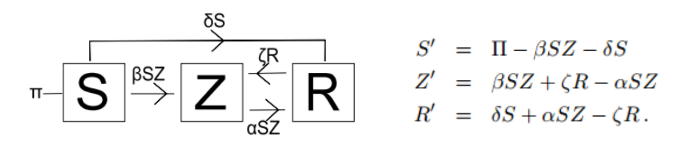
\includegraphics[scale=0.3]{ecz1.png}
\end{center}

El c\'odigo qued\'o de la siguiente manera: 

\begin{verbatim}
import numpy as gatito
import matplotlib.pyplot as plt
from scipy.integrate import odeint
plt.ion()
plt.rcParams['figure.figsize'] = 10, 8

Pi = 0        # Nacimientos Diarios
Del = 0.0001  # Muertes Naturales %  (Por dia)
Bet = 0.0095  # Transmision       %  (Por dia)
Zet = 0.0001  # Removidos         %  (Por dia)
Alf = 0.005   # Destruidos        %  (Por dia)

#Sistema de Ecuaciones Diferenciales 
def f(y, t):
    Si = y[0]
    Zi = y[1]
    Ri = y[2]
    # Modelo 
    f0 = Pi - Bet*Si*Zi - Del*Si              #Si
    f1 = Bet*Si*Zi + Zet*Ri - Alf*Si*Zi       #Zi 
    f2 = Del*Si + Alf*Si*Zi - Zet*Ri          #Ri
    return [f0, f1, f2]

S0 = 500.                        # Poblacion Inicial
Z0 = 0                           # Zombie Inicial
R0 = 0                           # Muertos Inicial
y0 = [S0, Z0, R0]                # Condicion Inicial
t  = gatito.linspace(0, 14., 1000)   #Tiempo

# Solucion E.D
soln = odeint(f, y0, t)
S = soln[:, 0]
Z = soln[:, 1]
R = soln[:, 2]
# Grafica
plt.figure()
plt.ylim(0,600)
plt.grid(True)
plt.plot(t, S, label='Vivos')
plt.plot(t, Z, label='Zombies')
plt.xlabel('Tiempo')
plt.ylabel('Poblacion')
plt.title('Apocalipsis Zombie - Modelo Basico')
plt.legend(loc="best")
\end{verbatim}

Las gr\'aficas resultantes son las siguientes:

\begin{center}

\begin{tabular}{c c}
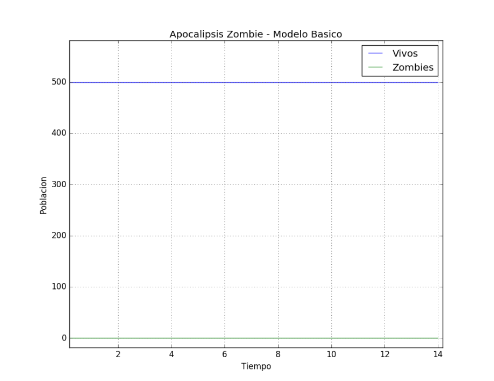
\includegraphics[scale=0.6]{graz1.png} & 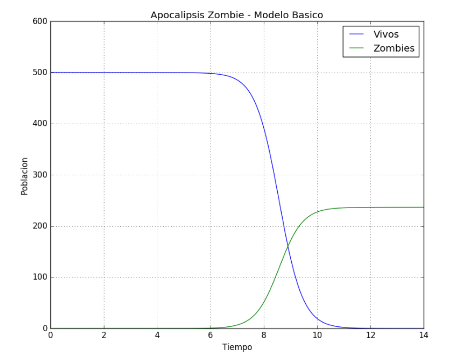
\includegraphics[scale=0.6]{graz11.png}\\
Caso sin Zombies SZR & Modelo B\'asico SZR
\end{tabular}

\end{center}

\subsection*{Modelo con infecci\'on latente (SIZR)}
En este modelo incluimos el efecto causado por una clase de infectados. Ahora se considera un tiempo de incubaci\'on y el efecto de este virus en una persona infectada, esta nueva clase modifica a la poblaci\'on Z directamente, pero lo retarda el tiempo en que S se transforma a Z. 

Ecuaciones:
\begin{center}
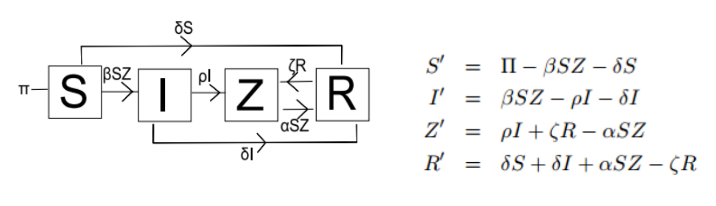
\includegraphics[scale=0.3]{ecz2.png}
\end{center}

C\'odigo: 
\begin{verbatim}
import numpy as gatito
import matplotlib.pyplot as plt
from scipy.integrate import odeint
plt.ion()
plt.rcParams['figure.figsize'] = 10, 8

Pi = 0         # Nacimientos Diarios
Del = 0.0001   # Muertes Naturales %  (Por dia)
Bet = 0.0095   # Transmision       %  (Por dia)
Zet = 0.0001   # Removidos         %  (Por dia)
Alf = 0.0001   # Destruidos        %  (Por dia)
Rho = 0.05     # Infected          %  (Por dia)

#Sistema de Ecuaciones Diferenciales 
def f(y, t):
    Si = y[0]
    Zi = y[1]
    Ri = y[2]
    Ii = y[3]
    # Modelo
    f0 = Pi - Bet*Si*Zi - Del*Si                #Si
    f1 = Rho*Ii + Zet*Ri - Alf*Si*Zi            #Zi
    f2 = Del*Si + Del*Ii + Alf*Si*Zi - Zet*Ri   #Ri
    f3 = Bet*Si*Zi -Rho*Ii - Del*Ii             #Ii
    
    return [f0, f1, f2, f3]

S0 = 500.                        # Poblacion Inicial
Z0 = 0.                          # Zombie Inicial
R0 = 0.                          # Muertos Inicial
I0 = 1.                          # Infectados Inicial
y0 = [S0, Z0, R0, I0]            # Condiciones Iniciales
t  = gatito.linspace(0., 30., 1000)  # Tiempo

# Solucion E.D.
soln = odeint(f, y0, t)
S = soln[:, 0]
Z = soln[:, 1]
R = soln[:, 2]
I = soln[:, 3]
# Grafica
plt.figure()
plt.ylim(0,600)
plt.grid(True)
plt.plot(t, S, label='Vivos')
plt.plot(t, Z, label='Zombies')
plt.xlabel('Tiempo')
plt.ylabel('Poblacion')
plt.title('Apocalipsis Zombie - Modelo Latente.')
plt.legend(loc="best")
\end{verbatim}

\newpage
La gr\'afica del modelo B\'asico SIZR qued\'o de la siguiente manera:

\begin{center}
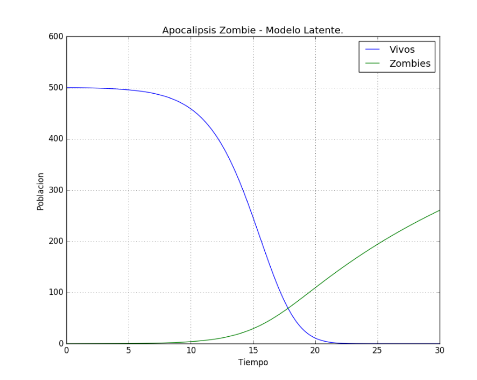
\includegraphics[scale=0.6]{graz2.png} 
\end{center}

\subsection*{Modelo Cuarentena (SIZRQ)}
Para poder contener el brote, se separan a los infectados y se les pone en cuarentena, (tambi\'en a unos cuantos zombies). Pero existe la posibilidad de que estos individuos en cuarentena intenten escapar y que los maten antes de que lo logren o que mueran en cuarentena. 

Ecuaciones:
\begin{center}
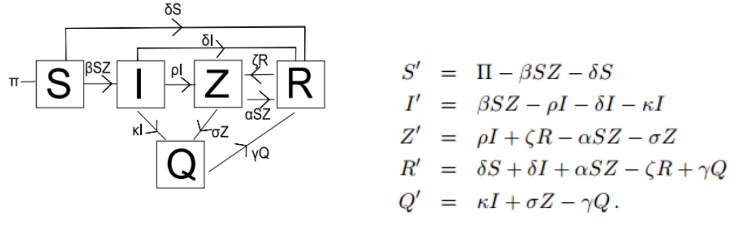
\includegraphics[scale=0.3]{ecz3.png}
\end{center}

C\'odigo modificado:
\begin{verbatim}
# zombie apocalypse modeling
import numpy as gatito
import matplotlib.pyplot as plt
from scipy.integrate import odeint
plt.ion()
plt.rcParams['figure.figsize'] = 10, 8

Pi = 0         # Nacimientos Diarios
Del = 0.0001   # Muertes Naturales %  (Por dia)
Bet = 0.0095   # Transmision       %  (Por dia)
Zet = 0.0001   # Removidos         %  (Por dia)
Alf = 0.0001   # Destruidos        %  (Por dia)
Rho = 0.05     # Infected          %  (Por dia)
Kap = 0.15     # Infectados Q      %  (Por dia)
Sig = 0.10     # Infected          %  (Por dia)
Gam = 0.001    # Infected          %  (Por dia)

#Sistema de Ecuaciones Diferenciales 
def f(y, t):
    Si = y[0]
    Zi = y[1]
    Ri = y[2]
    Ii = y[3]
    Qi = y[4]
    # Modelo
    f0 = Pi - Bet*Si*Zi - Del*Si                        #Si
    f1 = Rho*Ii + Zet*Ri - Alf*Si*Zi - Sig*Zi           #Zi
    f2 = Del*Si + Del*Ii + Alf*Si*Zi - Zet*Ri + Gam*Qi  #Ri
    f3 = Bet*Si*Zi -Rho*Ii - Del*Ii - Kap*Ii            #Ii
    f4 = Kap*Ii + Sig*Zi - Gam*Qi                       #Qi
    return [f0, f1, f2, f3, f4]

S0 = 500.                        # Poblacion Inicial
Z0 = 0.                          # Zombie Inicial
R0 = 0.                          # Muertos Inicial
I0 = 1.                          # Infectados Inicial
Q0 = 0.				 # Cuarentena Inicial
y0 = [S0, Z0, R0, I0, Q0]        # Condiciones Iniciales
t  = gatito.linspace(0., 30., 1000)  # Tiempo

# Solucion E.D.
soln = odeint(f, y0, t)
S = soln[:, 0]
Z = soln[:, 1]
R = soln[:, 2]
I = soln[:, 3]
Q = soln[:, 4]
# Grafica
plt.figure()
plt.ylim(0,600)
plt.grid(True)
plt.plot(t, S, label='Vivos')
plt.plot(t, Z, label='Zombies')
plt.xlabel('Tiempo')
plt.ylabel('Poblacion')
plt.title('Apocalipsis Zombie - Modelo Caurentena.')
plt.legend(loc="best")
\end{verbatim}

\newpage
La gr\'afica del modelo B\'asico SIZRQ qued\'o de la siguiente manera:

\begin{center}
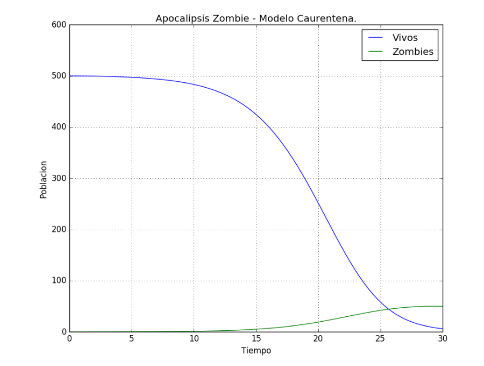
\includegraphics[scale=0.6]{graz3.png} 
\end{center}

\subsection*{Modelo Cura}
Aqu\'i se suponemos que se puede producir una cura, la cual permitir\'ia transformar a los zombies en humanos nuevamente, suponemos tambi\'en, que la cura no los vuelve inmunes y se descarta la cuarentena.

Ecuaciones: 

\begin{center}
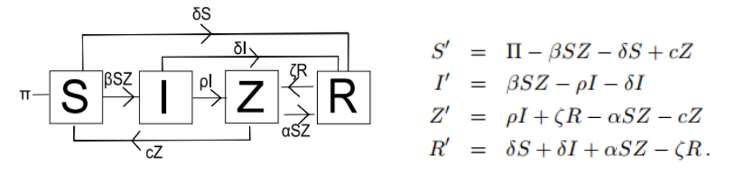
\includegraphics[scale=0.3]{ecz4.png}
\end{center}

C\'odigo:
\begin{verbatim}
import numpy as gatito
import matplotlib.pyplot as plt
from scipy.integrate import odeint
plt.ion()
plt.rcParams['figure.figsize'] = 10, 8

Pi  = 0        # Nacimientos Diarios
Del = 0.0001   # Muertes Naturales %  (Por dia)
Bet = 0.0095   # Transmision       %  (Por dia)
Zet = 0.0001   # Removidos         %  (Por dia)
Alf = 0.0001   # Destruidos        %  (Por dia)
Rho = 0.05     # Infected          %  (Por dia)
Ce  = 0.05     # Cura              %  (Por dia)

#Sistema de Ecuaciones Diferenciales 
def f(y, t):
    Si = y[0]
    Zi = y[1]
    Ri = y[2]
    Ii = y[3]
    # Modelo
    f0 = Pi - Bet*Si*Zi - Del*Si +Ce*Zi             #Si
    f1 = Rho*Ii + Zet*Ri - Alf*Si*Zi -Ce*Zi         #Zi
    f2 = Del*Si + Del*Ii + Alf*Si*Zi - Zet*Ri       #Ri
    f3 = Bet*Si*Zi -Rho*Ii - Del*Ii                 #Ii
    
    return [f0, f1, f2, f3]

S0 = 500.                        # Poblacion Inicial
Z0 = 0.                          # Zombie Inicial
R0 = 0.                          # Muertos Inicial
I0 = 1.                          # Infectados Inicial
y0 = [S0, Z0, R0, I0]            # Condiciones Iniciales
t  = gatito.linspace(0., 30., 1000)  # Tiempo

# Solucion E.D.
soln = odeint(f, y0, t)
S = soln[:, 0]
Z = soln[:, 1]
R = soln[:, 2]
I = soln[:, 3]
# Grafica
plt.figure()
plt.ylim(0,500)
plt.grid(True)
plt.plot(t, S, label='Vivos')
plt.plot(t, Z, label='Zombies')
plt.xlabel('Tiempo')
plt.ylabel('Poblacion')
plt.title('Apocalipsis Zombie - Modelo Tratamiento.')
plt.legend(loc="best")
\end{verbatim}

\newpage
La gr\'afica del modelo B\'asico SIZR con cura qued\'o de la siguiente manera:

\begin{center}
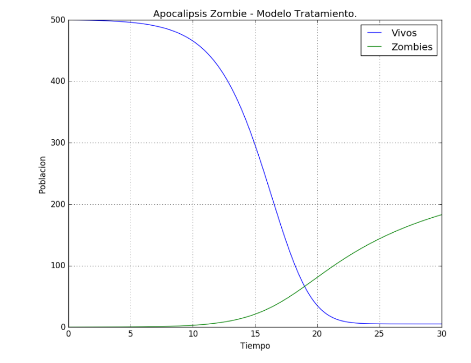
\includegraphics[scale=0.6]{graz4.png} 
\end{center}





\begin{thebibliography}{widestlabel}
      \bibitem{1} Zombiepedia, \emph{Variedad de Zombies}, (2016, 01 de Mayo).Desde: \url{http://zombie.wikia.com/wiki/Zombie_Wiki}
      \bibitem{2} SciPy Cookbook, \emph{Modeling a Zombie Apocalypse}, (2016, 01 de Mayo).Desde: \url{http://scipy-cookbook.readthedocs.io/items/Zombie_Apocalypse_ODEINT.html}
\end{thebibliography}


\end{document}